%% Draft manuscript. The journal-specific Springer class can be selected after
%% the target journal is fixed; the current class is retained for a portable build.
%% Fonts: newtx for text and mathematics; Source Code Pro for source listings.
\documentclass[preprint,12pt]{elsarticle}

\usepackage{amsmath}
\usepackage{amssymb}
\usepackage{newtxtext}
\usepackage{newtxmath}
\usepackage{graphicx}
\usepackage{booktabs}
\usepackage{array}
\usepackage{algorithm}
\usepackage{algpseudocode}
\usepackage{xcolor}
\usepackage{listings}
\usepackage{tcolorbox}
\tcbuselibrary{listings}
\usepackage[scale=0.90]{sourcecodepro}
\usepackage[colorlinks=true,linkcolor=blue,citecolor=blue,urlcolor=blue]{hyperref}
\usepackage{xurl}


% ---- Notation macros ----
\newcommand{\E}{\mathbb{E}}
\newcommand{\Normal}{\mathcal{N}}
\newcommand{\alphabar}{\bar{\alpha}}
\newcommand{\qhat}{\hat{\mathbf{q}}_0}

% ---- Source-code listings ----
\definecolor{draculaBackground}{HTML}{282A36}
\definecolor{draculaCurrentLine}{HTML}{44475A}
\definecolor{draculaForeground}{HTML}{F8F8F2}
\definecolor{draculaComment}{HTML}{6272A4}
\definecolor{draculaCyan}{HTML}{8BE9FD}
\definecolor{draculaPink}{HTML}{FF79C6}
\definecolor{draculaYellow}{HTML}{F1FA8C}
\lstdefinestyle{diffusionsdepython}{
  language=Python,
  basicstyle=\ttfamily\small\color{draculaForeground},
  keywordstyle=\bfseries\color{draculaPink},
  commentstyle=\itshape\color{draculaComment},
  stringstyle=\color{draculaYellow},
  emph={DiffusionConfig,DDPM},
  emphstyle=\bfseries\color{draculaCyan},
  frame=none,
  breaklines=true,
  columns=fullflexible,
  keepspaces=true,
  showstringspaces=false,
  tabsize=4,
  aboveskip=0pt,
  belowskip=0pt,
}
\newtcblisting{pythonlisting}{
  listing engine=listings,
  listing only,
  listing options={style=diffusionsdepython},
  colback=draculaBackground,
  colframe=draculaCurrentLine,
  boxrule=0.4pt,
  arc=0pt,
  boxsep=0pt,
  left=4pt,
  right=4pt,
  top=4pt,
  bottom=4pt,
  before skip=0pt,
  after skip=\baselineskip,
}

% ---- Figure placeholder for the first draft ----
\newcommand{\figbox}[1]{%
  \fbox{\parbox[c][5.5cm][c]{0.9\linewidth}{\centering\itshape [#1]}}}

% ---- Reference list environment used inside the Program Summary ----
\newcounter{bla}
\newenvironment{refnummer}{%
\list{[\arabic{bla}]}%
{\usecounter{bla}%
 \setlength{\itemindent}{0pt}%
 \setlength{\topsep}{0pt}%
 \setlength{\itemsep}{0pt}%
 \setlength{\labelsep}{2pt}%
 \setlength{\listparindent}{0pt}%
 \settowidth{\labelwidth}{[9]}%
 \setlength{\leftmargin}{\labelwidth}%
 \addtolength{\leftmargin}{\labelsep}%
 \setlength{\rightmargin}{0pt}}}
 {\endlist}

\begin{document}

\begin{frontmatter}

\title{\texttt{diffusionsde}: conditional diffusion models for stochastic dynamical systems}

\author[a]{Jack Griffiths}
\ead{jack.griffiths@sheffield.ac.uk}
\address[a]{School of Computer Science, Sheffield University, United Kingdom}

\author[b]{Matthew O. A. Ellis\corref{cor1}}
\ead{m.o.a.ellis@sheffield.ac.uk}
\cortext[cor1]{Corresponding author.}
\address[b]{School of Computer Science, Sheffield University, United Kingdom}

\begin{abstract}
A stochastic dynamical system defines a probability distribution over trajectories. We present \texttt{diffusionsde}, a Python package that creates generative models of dynamical systems from simulated or measured ensembles using diffusion modelling \cite{sohldickstein2015,ho2020ddpm,song2021ddim}. The package supports ancestral DDPM sampling and reduced-step DDIM sampling. With $\eta=0$ and fixed initial noise, the DDIM update can be made deterministic. Trajectories may be conditioned on initial conditions, external forcing, other time-dependent signals, or nothing at all. Once a model is learnt, it can be used to generate new trajectories given only the conditioning signal (e.g., to create a set of realistic trajectories given a set of initial conditions, or an external forcing waveform). The package also supports downstream tasks that rely upon the differentiability of the generative model, such as the inverse problem: given a set of trajectories, what was the conditioning signal that generated them? The package is designed to be agnostic to the underlying system, and it is therefore applicable to both simulated and measured data. We present three examples of increasing complexity to illustrate the package's capabilities: an Ornstein--Uhlenbeck process, a stochastically forced Duffing oscillator, and two experimental magnetic-reservoir-computing systems (for which a trusted governing equation is not available).

\end{abstract}

\begin{keyword}
diffusion model \sep stochastic processes \sep dynamical systems \sep generative
modelling \sep time series \sep inverse problems \sep Python
\end{keyword}

\end{frontmatter}

\section{Introduction}
\label{sec:introduction}

Many physical systems are intrinsically stochastic. Thermal fluctuations, environmental noise, unresolved degrees of freedom, and random forcing mean that repeated experiments or simulations performed under nominally identical conditions need not produce the same trajectory. The modelling problem is therefore to characterise this distribution for any arbitrary stochastic system. Direct numerical simulation provides samples from this distribution when the governing dynamics are known, but repeated simulation can become expensive when large ensembles are required across many parameter values.

Data-driven generative models provide an alternative. Neural stochastic differential equations represent stochastic dynamics through learned drift and diffusion functions \cite{kidger2021neuralsde}. In previous work, our group used neural SDEs to model the dynamics of experimental magnetic systems \cite{manneschi2025}. However, adversarial training of such models can be difficult, and generated ensembles may fail to reproduce the full variability of the data. Here we instead consider diffusion models, which learn a distribution through a (simpler) denoising objective rather than adversarial optimisation. In a denoising diffusion probabilistic model (DDPM), training trajectories are progressively corrupted with Gaussian noise and a neural network is trained to predict the added noise \cite{sohldickstein2015,ho2020ddpm}. Generation reverses this process to produce new samples from the learned distribution.

We introduce \texttt{diffusion}, an open-source Python package for conditional diffusion modelling of stochastic dynamical systems. Given simulated or measured trajectories and optional conditioning variables, the package learns
\begin{equation}
    p_{\phi}(\mathbf{x}_{0:T}\mid\mathbf{c})
    \approx
    p_{\mathrm{data}}(\mathbf{x}_{0:T}\mid\mathbf{c}).
\end{equation}
Conditioning $\mathbf{c}$ may include physical parameters, initial conditions, or time-dependent driving signals (or, indeed, nothing at all, in which case the model just samples from the learned distribution). The package supports DDPM and reduced-step DDIM sampling \cite{song2021ddim} (for faster inference), scalar and multichannel trajectories (to learn e.g., spectrograms), and dilated one-dimensional convolutional networks for very long time series or those with long-time correlations. Deterministic DDIM sampling may also be differentiated with respect to the conditioning variables, allowing the trained model to be used for gradient-based inverse problems (e.g., given a set of trajectories, estimate the conditioning variables that best explain the observed data).

We validate on four systems of increasing complexity, from a pure stochastic process to an experimental substrate: (i) the Ornstein–Uhlenbeck process, which provides a baseline with closed-form moments and autocorrelation; (ii) a driven stochastic Duffing oscillator with combined white and coloured noise, which is non-linear, stochastic, and potentially chaotic, and is conditioned on the driving field amplitude; (iii) a magnetic domain-wall oscillator~\cite{ababei2021} in the collective-coordinate model, which is phenomenologically Duffing-like, conditioned on the full driving field; (iv) an experimental interconnected nanomagnetic ring array~\cite{vidamour2022}, conditioned on a rotating in-plane field.

Whilst the package is agnostic to the underlying system, the examples illustrate a range of experimental substrates of interest to our group in the field of physical reservoir computing.
% ===========================================================================
% Problem formulation and methodology
% ===========================================================================

\section{Problem formulation and data representation}
\label{sec:physical_problem}

We consider stochastic dynamical systems with physical state
$\mathbf{x}(t)\in\mathbb{R}^m$. Its components $x_i(t)$ satisfy
\begin{equation}
    \mathrm{d}x_i
    =
    f_i(\mathbf{x},t;\boldsymbol{\lambda})\,\mathrm{d}t
    +
    \sum_{j=1}^{m_W}
    G_{ij}(\mathbf{x},t;\boldsymbol{\lambda})\,\mathrm{d}W_j,
    \qquad i=1,\ldots,m .
    \label{eq:generic_sde_component}
\end{equation}
Equivalently, $\mathrm{d}\mathbf{x}=\mathbf{f}(\mathbf{x},t;
\boldsymbol{\lambda})\,\mathrm{d}t+\mathbf{G}(\mathbf{x},t;
\boldsymbol{\lambda})\,\mathrm{d}\mathbf{W}$. Here $\mathbf{f}$ is the
drift, $\boldsymbol{\lambda}$ is a vector of physical parameters,
$\mathbf{G}\in\mathbb{R}^{m\times m_W}$ is the diffusion matrix, and $m_W$ is
the number of independent Wiener processes collected in
$\mathbf{W}(t)\in\mathbb{R}^{m_W}$. A state-independent
$\mathbf{G}$ gives additive noise, whereas a state-dependent $\mathbf{G}$
gives multiplicative noise. The simulated examples in this paper use additive
noise. A coloured random force can be represented by an augmented state with its
own stochastic dynamics; this construction is used for the Duffing oscillator in
Section~\ref{ssec:duffing}.

All SDEs in this manuscript use the It\^o convention. For the additive-noise
examples, the It\^o and Stratonovich forms are identical.

The package does not require Eq.~\eqref{eq:generic_sde_component} during
training. It requires an ensemble of observed trajectories and conditioning data.
For each sample $s$ of an ensemble of size $N_S$, the stored observable and
conditioning tensor are
\begin{equation}
    \mathbf{q}^{(s)}\in\mathbb{R}^{C_q\times N_T},
    \qquad
    \mathbf{c}^{(s)}\in\mathbb{R}^{C_c\times N_T},
    \label{eq:trajectory_conditioning_tensors}
\end{equation}
where $C_q$ is the number of generated channels, $C_c$ is the number of
conditioning channels, and $N_T$ is the number of physical-time samples. For a
scalar signal the channel axis can be omitted, giving tensors of shape
$[N_S,N_T]$. A conditioning channel can contain a constant parameter, an initial
state encoded at leading positions and zero-padded, or a full waveform sampled on
the same grid as the trajectory. This representation permits the same network to
handle stationary processes, initial-value problems, and driven systems.

The observable $\mathbf{q}$ can be the full physical state $\mathbf{x}$ or a
measured component of it. We use $t$ for continuous physical time, $n$ for a
physical-time index, $k$ for an artificial diffusion index, $s$ for an ensemble
member, and $a$ for a signal channel. Bold symbols denote vectors or tensors. The
identity matrix $\mathsf{I}$ has the dimension required by its context.

For a specified condition $\mathbf{c}$, repeated realisations define a
conditional path distribution,
\begin{equation}
    \mathbf{q}\sim p_{\mathrm{data}}(\mathbf{q}\mid\mathbf{c}).
    \label{eq:physical_trajectory_distribution}
\end{equation}
The model seeks
$p_\phi(\mathbf{q}\mid\mathbf{c})\approx
p_{\mathrm{data}}(\mathbf{q}\mid\mathbf{c})$. Validation therefore compares
time-dependent moments, correlations, spectra, and marginal distributions rather
than individual paths. The symbol $\phi$ denotes the trainable network parameters.

Preprocessing is applied after splitting the dataset. In the supplied numerical
workflows, every generated channel is standardised with statistics from the
training set,
\begin{equation}
    q_{a,n}^{\mathrm{sc},(s)}
    =
    \frac{q_{a,n}^{(s)}-\mu_a^{\mathrm{train}}}
         {\sigma_a^{\mathrm{train}}},
    \qquad
    a=1,\ldots,C_q,\quad n=0,\ldots,N_T-1,
    \label{eq:standardisation}
\end{equation}
where $\mu_a^{\mathrm{train}}$ and $\sigma_a^{\mathrm{train}}>0$ are computed over
the training samples and physical-time positions in channel $a$. Generated samples
are returned to physical units before validation. The same rule applies to
conditioning variables when they are scaled. The package leaves these transforms
outside the model. A user can preserve units, apply a logarithmic transform, or use
a problem-specific representation without changing the denoiser. Unless stated
otherwise, $\mathbf{q}$ and $\mathbf{c}$ in the diffusion equations below denote
these model-scale tensors. For a generated channel, the inverse transform is
\begin{equation}
    q_{a,n}^{(s)}
    =
    \sigma_a^{\mathrm{train}}q_{a,n}^{\mathrm{sc},(s)}
    +
    \mu_a^{\mathrm{train}}.
    \label{eq:inverse_standardisation}
\end{equation}
Thus, \texttt{DDPM.generate} returns model-scale data, and the caller applies
Eq.~\eqref{eq:inverse_standardisation} before validation in physical units. For a
zero-padded conditioning tensor, transform the physical value before placing it in
the tensor. Do not standardise the padded tensor after adding zeros.

The \texttt{train\_dataset} argument in the minimal interface stores the
observable first and the condition second. The example below has one generated
channel and one conditioning channel. Multichannel tensors retain the channel
axis defined in Eq.~\eqref{eq:trajectory_conditioning_tensors}.

\begin{pythonlisting}
from torch.utils.data import TensorDataset

# Shape: [n_trajectories, n_time]
train_dataset = TensorDataset(trajectories, conditioning)
\end{pythonlisting}


% ===========================================================================
% Conditional diffusion model
% ===========================================================================

\section{Conditional diffusion method}
\label{sec:conditional_diffusion}

The generator is a conditional denoising diffusion probabilistic model (DDPM)
\cite{ho2020ddpm}. The diffusion index $k$ is an artificial coordinate and is
distinct from physical time $t$. Starting from the clean model-scale trajectory
$\mathbf{q}_0\equiv\mathbf{q}$, the forward process adds Gaussian noise. A neural
network predicts that noise from $(\mathbf{q}_k,k,\mathbf{c})$.
Figure~\ref{fig:diffusion_highlevel} shows this separation between physical data
and the artificial diffusion process.

\begin{figure}[t]
    \centering
    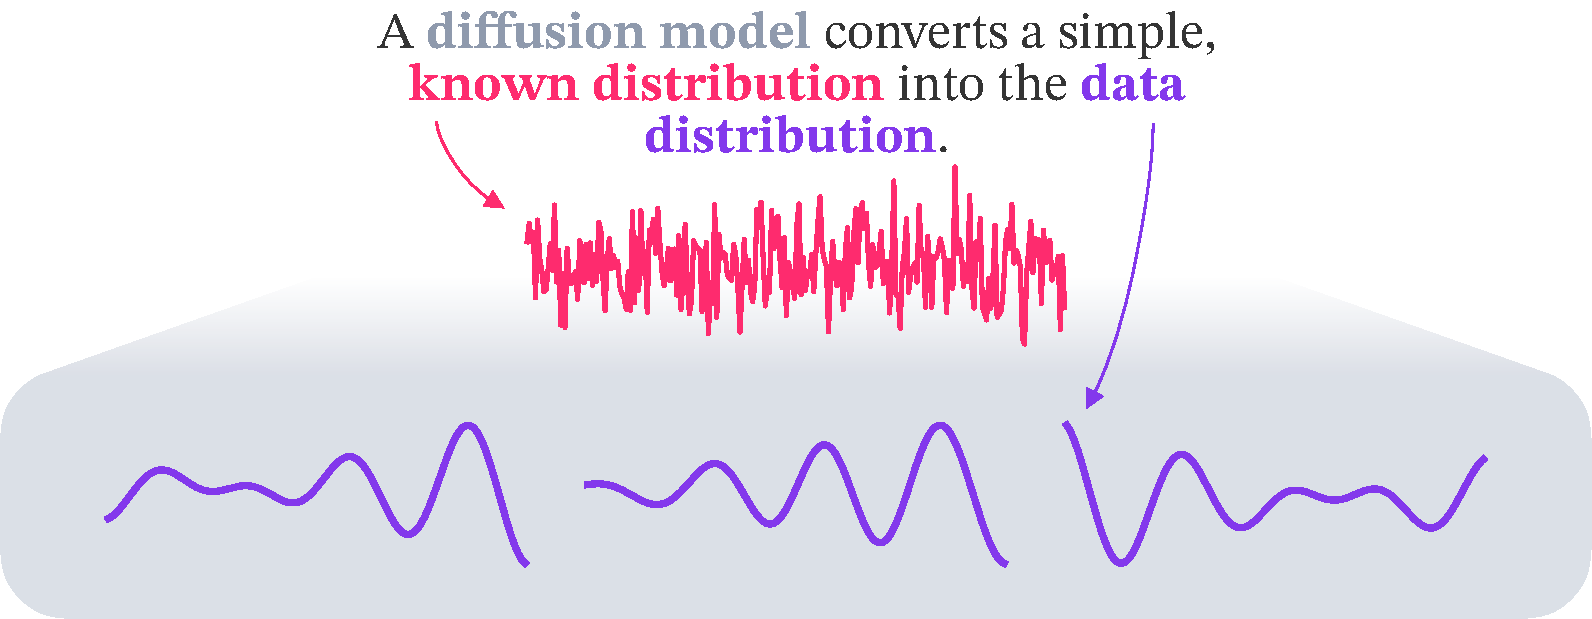
\includegraphics[width=0.8\textwidth]{diffusion_highlevel.pdf}
    \caption{Conditional diffusion model for stochastic trajectories. During
    training, model-scale trajectory tensors are corrupted by artificial Gaussian
    noise and a neural network predicts that noise. Generation starts from a
    standard Gaussian sampling prior and applies the learned reverse process. The
    conditioning variables select the trajectory distribution to be sampled.}
    \label{fig:diffusion_highlevel}
\end{figure}

\subsection{Forward process and training objective}
\label{ssec:fit}

Let $N_K\geq2$ be the number of diffusion steps. We use $k=0,\ldots,N_K$, where
$k=0$ denotes clean data. The implementation uses the linear schedule
\begin{equation}
  \begin{aligned}
    \beta_k
    =
    \beta_1+\frac{k-1}{N_K-1}(\beta_{N_K}-\beta_1),
    \qquad 0<\beta_1\leq\beta_{N_K}<1,
    \qquad k=1,\ldots,N_K,
    \\
    \alphabar_0=1,
    \qquad
    \alpha_k=1-\beta_k,
    \qquad
    \alphabar_k=\prod_{\ell=1}^{k}\alpha_\ell .
  \end{aligned}
    \label{eq:alpha_schedule}
\end{equation}
The forward Markov transition is
\begin{equation}
    \mathbf{q}_k
    =
    \sqrt{\alpha_k}\,\mathbf{q}_{k-1}
    +
    \sqrt{\beta_k}\,\boldsymbol{\varepsilon}_k,
    \qquad
    \boldsymbol{\varepsilon}_k\sim\Normal(\mathbf{0},\mathsf{I}).
    \label{eq:forward_step}
\end{equation}
Repeated substitution multiplies $\mathbf{q}_0$ by
$\prod_{\ell=1}^{k}\sqrt{\alpha_\ell}$. The independent Gaussian increments
combine into one Gaussian tensor with variance $(1-\alphabar_k)\mathsf{I}$.
This gives the closed-form marginal
\begin{equation}
    p_{\mathrm{fwd}}(\mathbf{q}_k\mid\mathbf{q}_0)
    =
    \Normal\!\left(
        \mathbf{q}_k;
        \sqrt{\alphabar_k}\,\mathbf{q}_0,
        (1-\alphabar_k)\mathsf{I}
    \right),
    \label{eq:forward_marginal_density}
\end{equation}
so a noisy sample at any diffusion index is drawn directly as
\begin{equation}
    \mathbf{q}_k
    =
    \sqrt{\alphabar_k}\,\mathbf{q}_0
    +
    \sqrt{1-\alphabar_k}\,\boldsymbol{\varepsilon},
    \qquad
    \boldsymbol{\varepsilon}\sim\Normal(\mathbf{0},\mathsf{I}).
    \label{eq:forward_marginal}
\end{equation}
Only one sampled diffusion index and one noise tensor are therefore needed for a
training example. The code stores diffusion indices as $r=0,\ldots,N_K-1$; code
index $r$ corresponds to the paper index $k=r+1$.

The denoiser $\boldsymbol{\varepsilon}_\phi(\mathbf{q}_k,k,\mathbf{c})$
predicts the perturbation in Eq.~\eqref{eq:forward_marginal}. For each training
pair $(\mathbf{q}_0,\mathbf{c})$, the implementation samples
$k\sim\mathrm{Unif}\{1,\ldots,N_K\}$ and
$\boldsymbol{\varepsilon}\sim\Normal(\mathbf{0},\mathsf{I})$. These draws are
independent across a minibatch. The noise-prediction objective is
\begin{equation}
    \mathcal{L}(\phi)
    =
    \E
    \left[
        \frac{1}{C_qN_T}
        \left\|
            \boldsymbol{\varepsilon}
            -
            \boldsymbol{\varepsilon}_\phi
            (\mathbf{q}_k,k,\mathbf{c})
        \right\|_F^2
    \right].
    \label{eq:noise_objective}
\end{equation}
Minibatches estimate the expectation. Mean-squared error (MSE) is the default
loss; Huber loss is available for data with large residuals.
Differentiating the log of
Eq.~\eqref{eq:forward_marginal_density} gives the score of the forward kernel for
a fixed clean trajectory,
\begin{equation}
    \nabla_{\mathbf{q}_k}
    \log p_{\mathrm{fwd}}(\mathbf{q}_k\mid\mathbf{q}_0)
    =
    -\frac{\boldsymbol{\varepsilon}}
            {\sqrt{1-\alphabar_k}}.
    \label{eq:conditional_score}
\end{equation}
Let $p_k(\mathbf{q}_k\mid\mathbf{c})$ denote the conditional noisy-trajectory distribution
after $k$ forward steps. It is obtained by integrating out the clean trajectory,
\begin{equation}
    p_k(\mathbf{q}_k\mid\mathbf{c})
    =
    \int p_{\mathrm{fwd}}(\mathbf{q}_k\mid\mathbf{q}_0)
    p_{\mathrm{data}}(\mathbf{q}_0\mid\mathbf{c})
    \,\mathrm{d}\mathbf{q}_0.
    \label{eq:conditional_noisy_density}
\end{equation}
Its score is the conditional mean of the forward-kernel score,
\begin{equation}
    \nabla_{\mathbf{q}_k}\log p_k(\mathbf{q}_k\mid\mathbf{c})
    =
    \E\!\left[
        \nabla_{\mathbf{q}_k}
        \log p_{\mathrm{fwd}}(\mathbf{q}_k\mid\mathbf{q}_0)
        \mathrel{\big|}\mathbf{q}_k,\mathbf{c}
    \right]
    =
    -\frac{\E[\boldsymbol{\varepsilon}\mid\mathbf{q}_k,\mathbf{c}]}
            {\sqrt{1-\alphabar_k}}.
    \label{eq:conditional_score_identity}
\end{equation}
With mean-squared error, the optimal predictor is
$\E[\boldsymbol{\varepsilon}\mid\mathbf{q}_k,\mathbf{c}]$. Replacing that
conditional mean by the fitted predictor gives
\begin{equation}
    -\frac{\boldsymbol{\varepsilon}_\phi(\mathbf{q}_k,k,\mathbf{c})}
           {\sqrt{1-\alphabar_k}}
    \approx
    \nabla_{\mathbf{q}_k}\log p_k(\mathbf{q}_k\mid\mathbf{c}).
    \label{eq:data_score}
\end{equation}
Thus the fitted noise predictor defines a conditional noisy-data score estimate
\cite{vincent2011connection,hyvarinen2005score}. This relation applies to the
mean-squared-error loss, not directly to the optional Huber loss.

\subsection{Conditional denoiser and fitting}

The denoiser is a one-dimensional residual U-Net \cite{ronneberger2015unet}.
For a minibatch,
\begin{equation}
    \mathbf{q}_k\in\mathbb{R}^{B\times C_q\times N_T},
    \qquad
    \mathbf{c}\in\mathbb{R}^{B\times C_c\times N_T}.
    \label{eq:denoiser_tensor_shapes}
\end{equation}
where $B$ is the minibatch size. The network concatenates these tensors along the
channel axis, embeds the
diffusion index with fixed
sinusoidal features \cite{vaswani2017attention}, and injects the embedding into
each residual block. Encoder blocks reduce the temporal resolution, a bottleneck
operates at the coarsest scale, and decoder blocks restore the original resolution
with skip connections. The final convolution returns a tensor with the same shape
as the generated trajectory.

Each residual block uses two convolutions, group normalisation
\cite{wu2018groupnorm}, SiLU activation, and a residual connection
\cite{he2016residual}. The channel width doubles with encoder depth. An optional
dilation schedule enlarges the temporal receptive field without increasing the
number of convolution weights. A fixed physical-position encoding can be added
after the input projection when absolute time or drive phase is physically
relevant. The optional causal mode uses left-only convolution padding, so a
prediction at one physical-time location cannot depend on later locations.

The configuration distinguishes physical trajectory length from the number of
artificial diffusion steps. This example sets the data shape and a 200-step DDIM
sampler with $\eta=0$, then calls \texttt{fit}.

\begin{pythonlisting}
from diffusionsde import DDPM, DiffusionConfig

config = DiffusionConfig(
    trajectory_length=n_time,
    n_output_channels=n_signal_channels,
    n_conditioning_channels=n_condition_channels,
)
model = DDPM(
    config,
    sampler_type="ddim",
    sampler_kwargs={"num_inference_steps": 200, "eta": 0.0},
)
history = model.fit(
    train_dataset,
    val_dataset=validation_dataset,
)
\end{pythonlisting}

Training uses Adam \cite{kingma2015adam}, cosine learning-rate annealing
\cite{loshchilov2017sgdr}, shuffled minibatches, and clipping of the global
gradient norm to unity. If a validation dataset is supplied, the model state with
the smallest validation loss is restored after training. The returned history
contains the training loss and, when applicable, the validation loss, best
validation loss, and best epoch.

Table~\ref{tab:config} lists the defaults that affect the numerical method. The
physical trajectory length is independent of $N_K$, the number of artificial
diffusion steps. The U-Net accepts other lengths; exact two-fold reductions occur
when the length is divisible by $2^{n_{\mathrm{layers}}-1}$.

\begin{table}[t]
  \centering
  \caption{Selected \texttt{DiffusionConfig} defaults.}
  \label{tab:config}
  \small
  \begin{tabular}{@{}lll@{}}
    \toprule
    Group & Entry & Default \\
    \midrule
    Diffusion & steps $N_K$ & $1000$ \\
    Diffusion & $(\beta_1,\beta_{N_K})$ & $(10^{-4},0.02)$ \\
    Data & trajectory length & $250$ \\
    Architecture & hidden width & $128$ \\
    Architecture & encoder levels & $4$ \\
    Optimisation & learning rate & $10^{-4}$ \\
    Optimisation & batch size, epochs & $32$, $50$ \\
    Loss & form & MSE; Huber optional \\
    \bottomrule
  \end{tabular}
\end{table}

The checkpoint stores the model and training state. \texttt{DDPM.load} restores
the configuration and weights for generation, but not the optimiser or scheduler.
Sampler type and sampler arguments are set when the model is constructed.

\subsection{Reverse sampling and generation}
\label{ssec:generate}

The schedule is selected so that the terminal forward marginal is close to a
standard Gaussian when $\alphabar_{N_K}\ll1$. The sampler therefore starts from
\begin{equation}
    \mathbf{q}_{N_K}\sim\Normal(\mathbf{0},\mathsf{I}).
    \label{eq:sampling_seed}
\end{equation}
For ancestral DDPM sampling, the forward chain defines the Gaussian posterior
$p_{\mathrm{fwd}}(\mathbf{q}_{k-1}\mid\mathbf{q}_k,\mathbf{q}_0)$. Substituting
the denoiser estimate for the unknown forward noise gives the learned reverse
transition for $k=2,\ldots,N_K$,
\begin{equation}
    p_\phi(\mathbf{q}_{k-1}\mid\mathbf{q}_k,\mathbf{c})
    =
    \Normal\!\left(
        \mathbf{q}_{k-1};
        \boldsymbol{\mu}_\phi(\mathbf{q}_k,k,\mathbf{c}),
        \widetilde{\beta}_k\mathsf{I}
    \right),
    \label{eq:ddpm_reverse_density}
\end{equation}
where
\begin{equation}
    \boldsymbol{\mu}_\phi(\mathbf{q}_k,k,\mathbf{c})
    =
    \frac{1}{\sqrt{\alpha_k}}
    \left[
        \mathbf{q}_k
        -
        \frac{\beta_k}{\sqrt{1-\alphabar_k}}
        \boldsymbol{\varepsilon}_\phi(\mathbf{q}_k,k,\mathbf{c})
    \right],
    \label{eq:ddpm_reverse_mean}
\end{equation}
and
\begin{equation}
    \widetilde{\beta}_k
    =
    \beta_k\frac{1-\alphabar_{k-1}}{1-\alphabar_k}.
    \label{eq:ddpm_reverse_variance}
\end{equation}
At $k=1$, $\widetilde{\beta}_1=0$, so the sampler uses the mean in
Eq.~\eqref{eq:ddpm_reverse_mean} and returns $\mathbf{q}_0$ without posterior
noise. The DDPM sampler evaluates every reverse index.

The package also implements denoising diffusion implicit model (DDIM) sampling
\cite{song2021ddim}. DDIM evaluates the denoiser at $S$ descending indices
\begin{equation}
    \kappa_0>\kappa_1>\cdots>\kappa_{S-1}\geq1,
    \qquad
    \kappa_S=0 .
    \label{eq:ddim_indices}
\end{equation}
For a transition from $\kappa_j$ to $\kappa_{j+1}$, with
$j=0,\ldots,S-1$, first form
\begin{equation}
    \widehat{\mathbf{q}}_0
    =
    \frac{
        \mathbf{q}_{\kappa_j}
        -
        \sqrt{1-\alphabar_{\kappa_j}}\,
        \boldsymbol{\varepsilon}_\phi(\mathbf{q}_{\kappa_j},\kappa_j,\mathbf{c})
    }{\sqrt{\alphabar_{\kappa_j}}}.
    \label{eq:ddim_q0}
\end{equation}
Equation~\eqref{eq:ddim_q0} follows by solving
Eq.~\eqref{eq:forward_marginal} for $\mathbf{q}_0$. The DDIM update retains the
predicted clean component, adds the denoising direction, and optionally adds a
new Gaussian tensor:
\begin{align}
    \sigma_j
    &=
    \eta
    \sqrt{\frac{1-\alphabar_{\kappa_{j+1}}}{1-\alphabar_{\kappa_j}}}
    \sqrt{1-\frac{\alphabar_{\kappa_j}}{\alphabar_{\kappa_{j+1}}}},
    \label{eq:ddim_sigma}\\
    \mathbf{q}_{\kappa_{j+1}}
    &=
    \sqrt{\alphabar_{\kappa_{j+1}}}\,\widehat{\mathbf{q}}_0
    +
    \sqrt{1-\alphabar_{\kappa_{j+1}}-\sigma_j^2}\,
    \boldsymbol{\varepsilon}_\phi(\mathbf{q}_{\kappa_j},\kappa_j,\mathbf{c})
    +
    \sigma_j\mathbf{z}_j,
    \qquad
    \mathbf{z}_j\sim\Normal(\mathbf{0},\mathsf{I}).
    \label{eq:ddim_update}
\end{align}
The parameter $0\leq\eta\leq1$ controls added noise. When $\eta=0$, a fixed
initial Gaussian tensor and a fixed condition define a deterministic generated
trajectory. Positive $\eta$ adds a new Gaussian tensor on each non-final reverse
transition for which $\sigma_j>0$. The final transition has $\sigma_j=0$ and
returns $\widehat{\mathbf{q}}_0$. When indices are skipped, $\eta=1$ remains a
DDIM update and is not the full ancestral DDPM chain.

The method \texttt{generate} expands each supplied condition to the requested
ensemble size. For $B$ conditions and $M$ samples per condition, it returns a
flat batch of $BM$ trajectories. The output shape is
\texttt{[BM, N\_T]} for $C_q=1$ and \texttt{[BM, C\_q, N\_T]} for
$C_q>1$. Output values remain on the model scale until the caller applies
Eq.~\eqref{eq:inverse_standardisation}.

The optional \texttt{initial\_noise} tensor supplies the initial
$\mathbf{q}_{N_K}$ in Eq.~\eqref{eq:sampling_seed}. With DDIM and $\eta=0$, the
same tensor and condition give the same output. The DDIM option
\texttt{require\_grad=True} retains the automatic-differentiation graph.
\texttt{grad\_steps} restricts gradient tracking to selected reverse steps. This
does not change the generated values, but the resulting gradient is approximate
and uses less memory.

\subsection{Statistical validation}
\label{ssec:evaluation}

The evaluator compares scalar ensembles with a sample axis and a physical-time
axis. It reports errors in the mean and standard-deviation curves. It also averages
the per-trajectory normalised autocorrelation and Welch power spectrum over the
ensemble \cite{welch1967psd}. Pooled tail statistics include skewness, excess
kurtosis, and the Wasserstein-1 distance \cite{villani2009optimal}. The argument
\texttt{tail\_fraction} selects the final part of each trajectory for the
autocorrelation, spectrum, and marginal tests.

\begin{pythonlisting}
from diffusionsde import StatisticsEvaluator

evaluator = StatisticsEvaluator(reference, generated)
metrics = evaluator.compute_extended_metrics(
    dt=dt, max_lag=64, tail_fraction=0.5,
)
\end{pythonlisting}

These tests are not interchangeable. Pointwise moments do not measure temporal
correlation, and a correct power spectrum does not imply a correct marginal
distribution. The sampling interval and selected tail must therefore be reported
with the metrics.

\subsection{Differentiable inverse estimation}
\label{ssec:inverse}

For differentiable parameter estimation, a fitted DDIM generator is used as a
conditional surrogate. The current solver treats scalar generated trajectories.
Let $\mathcal{I}$ be the physical-time indices used in the objective. For an
ensemble $e\in\{\mathrm{gen},\mathrm{obs}\}$ with $N_e>1$ trajectories, define
\begin{align}
  \overline{q}_n^e
  &= \frac{1}{N_e}\sum_{s=1}^{N_e}q_n^{e,(s)},
  \label{eq:ensemble_mean}\\
  V_n^e
  &= \frac{1}{N_e-1}\sum_{s=1}^{N_e}
  \left(q_n^{e,(s)}-\overline{q}_n^e\right)^2 .
  \label{eq:ensemble_variance}
\end{align}
The moment-matching objective is
\begin{equation}
  \mathcal{M}=\frac{w_{\mathrm{mean}}}{|\mathcal{I}|}
  \sum_{n\in\mathcal{I}}(\overline{q}_n^{\mathrm{gen}}-\overline{q}_n^{\mathrm{obs}})^2
  +\frac{w_{\mathrm{var}}}{|\mathcal{I}|}
  \sum_{n\in\mathcal{I}}(V_n^{\mathrm{gen}}-V_n^{\mathrm{obs}})^2 .
  \label{eq:moment_matching_loss}
\end{equation}
Both ensembles must use the same numerical scale. If $q$ has physical units,
$w_{\mathrm{mean}}$ has units $[q]^{-2}$ and $w_{\mathrm{var}}$ has units
$[q]^{-4}$ when $\mathcal{M}$ is dimensionless. Alternatively, the data can first
be nondimensionalised. For
\texttt{tail\_start=None}, $\mathcal{I}=\{0,\ldots,N_T-1\}$; otherwise it contains
the selected final interval. The objective does not replace the autocorrelation and
spectral checks. The solver uses differentiable DDIM generation and fixes one
initial Gaussian tensor during each optimisation restart. With $\eta=0$, this gives
a repeatable objective within the restart.

\begin{pythonlisting}
from diffusionsde import InverseProblem, InverseProblemConfig

def condition_from_parameter(p, n_gen, n_time, device, run_idx):
    return p.reshape(1, 1, 1).expand(n_gen, 1, n_time)

model.freeze()
inverse = InverseProblem(
    model, observed, condition_from_parameter, (p_min, p_max),
    InverseProblemConfig(n_iterations=100, n_gen=64),
)
result = inverse.solve(n_runs=8)
\end{pythonlisting}


% ===========================================================================
% Numerical verification
% ===========================================================================

\section{Numerical verification cases}
\label{sec:examples}

The two simulated systems test different properties. The Ornstein--Uhlenbeck
process has analytic continuous-time and exact discrete-time stationary statistics,
which permit direct checks of marginal and temporal fidelity. The driven Duffing
oscillator has nonlinear transients and coloured forcing, which test conditional
generation without a closed-form path distribution.

\subsection{Ornstein--Uhlenbeck process}
\label{ssec:ou}

The Ornstein--Uhlenbeck (OU) process \cite{uhlenbeck1930} obeys
\begin{equation}
    \mathrm{d}q
    =
    -\theta q\,\mathrm{d}t
    +
    \sqrt{2D}\,\mathrm{d}W,
    \label{eq:ou}
\end{equation}
where $\theta>0$ is the relaxation rate and $D>0$ is the diffusion coefficient.
For the continuous-time process, the stationary distribution and normalised
autocorrelation are
\begin{equation}
    q(t)\sim\Normal\!\left(0,\frac{D}{\theta}\right),
    \qquad
    \rho_{\mathrm{ct}}(\tau)=\exp(-\theta\lvert\tau\rvert).
    \label{eq:ou_continuous_stationary}
\end{equation}
The supplied notebook uses Euler--Maruyama rather than the exact OU transition.
With $t_n=n\Delta t$, its update is
\begin{equation}
    q_{n+1}=\varphi_\Delta q_n+\sqrt{2D\Delta t}\,z_n,
    \qquad
    \varphi_\Delta=1-\theta\Delta t,
    \qquad
    z_n\sim\Normal(0,1).
    \label{eq:ou_euler_update}
\end{equation}
For $0<\theta\Delta t<2$, let $V_\Delta=\operatorname{Var}(q_n)$ at
stationarity. Equation~\eqref{eq:ou_euler_update} gives
$V_\Delta=\varphi_\Delta^2V_\Delta+2D\Delta t$. Repeated application of the
same update gives the lag-$h$ correlation. The exact stationary references for
this discrete process are therefore
\begin{equation}
    q_n\sim\Normal\!\left(0,\frac{2D\Delta t}{1-\varphi_\Delta^2}\right),
    \qquad
    \rho_{\Delta}(h)=\varphi_\Delta^h,
    \qquad h=0,1,\ldots .
    \label{eq:ou_discrete_stationary}
\end{equation}
The variance tends to $D/\theta$ as $\Delta t\to0$. At a fixed physical lag
$\tau=h\Delta t$, $(1-\theta\Delta t)^h$ tends to $\exp(-\theta\tau)$.
Equation~\eqref{eq:ou_continuous_stationary} is therefore recovered in the
continuous-time limit. Equation~\eqref{eq:ou_discrete_stationary} is the strict
finite-step reference. Its variance tests the amplitude scale, and its
autocorrelation tests the relaxation time.

The supplied notebook samples $\theta\sim\mathcal{U}(0.8,3.0)$ and
$D\sim\mathcal{U}(0.1,1.5)$. Euler--Maruyama integration uses
$\Delta t=5/256$, discards $1024$ warm-up steps, and retains $N_T=256$ samples.
The training and held-out ensembles contain $512$ and $128$ trajectories,
respectively. The conditioning vector contains the training-set-standardised
values of $(\theta,D)$ in its first two entries and is zero elsewhere. The model
uses a two-level U-Net with hidden width $64$, $1000$ diffusion steps, and a
$200$-step DDIM sampler with $\eta=0$. These values replace the corresponding
defaults in Table~\ref{tab:config}; the training call is otherwise unchanged.

For each held-out parameter pair, the notebook generates one Euler--Maruyama
reference trajectory and one model trajectory. It then compares aggregate
statistics across all held-out conditions. For a finite-step reference, let
$\varphi_s=1-\theta_s\Delta t$. The pooled stationary marginal is the discrete
mixture
\begin{equation}
    p_{\mathrm{pool}}(q)
    =
    \frac{1}{N_{\mathrm{test}}}
    \sum_{s=1}^{N_{\mathrm{test}}}
    \Normal\!\left(q;0,\frac{2D_s\Delta t}{1-\varphi_s^2}\right),
    \label{eq:ou_pooled_mixture}
\end{equation}
with $N_{\mathrm{test}}=128$. The evaluator computes a normalised
autocorrelation for each trajectory and then averages it. The corresponding
condition-averaged reference is
\begin{equation}
    \overline{\rho}_{\mathrm{cond}}(h)
    =
    \frac{1}{N_{\mathrm{test}}}
    \sum_{s=1}^{N_{\mathrm{test}}}\varphi_s^h.
    \label{eq:ou_condition_average_acf}
\end{equation}
Equation~\eqref{eq:ou_condition_average_acf} is not the autocorrelation of the
pooled mixture. It is the mean of the population autocorrelations at the held-out
conditions and uses the same condition averaging as the evaluator. The finite
trajectory estimator is biased because it subtracts each trajectory mean, so exact
agreement with Eq.~\eqref{eq:ou_condition_average_acf} is not expected. This test
checks the collection of held-out conditions. It does not estimate a full
conditional distribution at one fixed $(\theta,D)$ pair; that test requires
repeated reference and model samples at the same condition.

\subsection{Driven Duffing oscillator}
\label{ssec:duffing}

The second case is a periodically driven Duffing oscillator with white and
coloured stochastic forcing. Introducing velocity $v$ and a coloured-force
variable $\xi$, the augmented system is
\begin{align}
    \mathrm{d}q
    &= v\,\mathrm{d}t,
    \label{eq:duffing_q}\\
    \mathrm{d}v
    &=
    \left[-\mu v-\alpha_{\mathrm{D}} q-\beta_{\mathrm{D}} q^3
    +\gamma\cos(\Omega t)+\xi\right]
    \mathrm{d}t
    +\sqrt{2\mu\Theta}\,\mathrm{d}W_1,
    \label{eq:duffing_v}\\
    \mathrm{d}\xi
    &=
    -\frac{\xi}{\tau_c}\,\mathrm{d}t
    +\sqrt{\frac{2D_\xi}{\tau_c}}\,\mathrm{d}W_2 .
    \label{eq:duffing_colour}
\end{align}
For the parameters below, the restoring force derives from the double-well
potential of the Duffing oscillator \cite{guckenheimer1983nonlinear}. Here $\mu$ is the damping
coefficient; $\alpha_{\mathrm{D}}$ and $\beta_{\mathrm{D}}$ define the linear and
cubic restoring force; $\gamma$ and $\Omega$ define the periodic drive; and $\Theta$ sets the
white-noise strength. The parameters $D_\xi$ and $\tau_c$ set the stationary
variance and correlation time of $\xi$. If $\xi$ is initialised from its
stationary distribution,
\begin{equation}
    \E[\xi(t)\xi(t+u)]
    =
    D_\xi\exp\!\left(-\frac{\lvert u\rvert}{\tau_c}\right).
    \label{eq:duffing_colour_covariance}
\end{equation}
where $u$ is a physical-time lag. The two Wiener processes are independent.

The notebook uses $\alpha_{\mathrm{D}}=-1$, $\beta_{\mathrm{D}}=1$, $\mu=0.3$, $\gamma=0.5$,
$\Omega=1.2$, $\Theta=0.05$, $\tau_c=0.5$, and $D_\xi=0.02$. These are the
nondimensional values of the numerical case; the source-code names
\texttt{alpha}, \texttt{beta}, and \texttt{D} correspond to
$\alpha_{\mathrm{D}}$, $\beta_{\mathrm{D}}$, and $D_\xi$, respectively. Initial values
$q_{\mathrm{init}}=q(0)$ and $v_{\mathrm{init}}=v(0)$ are sampled independently
from $\mathcal{U}(-1,1)$, while $\xi(0)=0$. The coloured force is therefore not
initially stationary; Eq.~\eqref{eq:duffing_colour_covariance} is its long-time
reference. A stochastic Heun update with $\Delta t=0.05$ produces trajectories
of length $N_T=256$. There are $1024$
training trajectories and $128$ held-out trajectories. The conditioning tensor
encodes $(q_{\mathrm{init}},v_{\mathrm{init}})$. It therefore defines a
conditional initial-value distribution, not a deterministic solution at one fixed
initial state.

The diffusion model uses four U-Net levels with hidden width $128$, $1000$
training diffusion steps, and a $200$-step DDIM sampler with $\eta=0.5$.
The nonzero value of $\eta$ adds noise on the non-final reverse transitions. Since
there is no closed-form trajectory distribution for this nonlinear driven system,
the held-out comparison uses representative paths, time-resolved means and
standard deviations, autocorrelation functions, power spectra, and pooled
position marginals. These diagnostics test different failures: correct moments do
not imply correct temporal correlations, and a correct spectrum does not imply a
correct marginal distribution.

The evaluator is applied after inverse standardisation. Section~\ref{ssec:evaluation}
defines its moment, correlation, spectral, and marginal tests. Both numerical cases
use the same \texttt{fit} and \texttt{generate} interface. OU supplies analytic
and finite-step references, while Duffing tests nonlinear transient dynamics with
coloured forcing.

\section{Experimental systems}\label{sec:experimental}

Both datasets of this section come from magnetic reservoir-computing hardware rather than from simulation. Neither system has a governing equation we trust enough to integrate numerically, which is precisely the regime the package targets. The trained surrogate therefore consumes the output of the raw measurement pipeline, subject only to the light preprocessing described below.

The same forward corruption, conditional denoiser and deterministic DDIM sampler developed through the OU example apply without change. The experimental cases differ only in their preprocessing, representation and conditioning design. 

\begin{figure}[h!]\centering
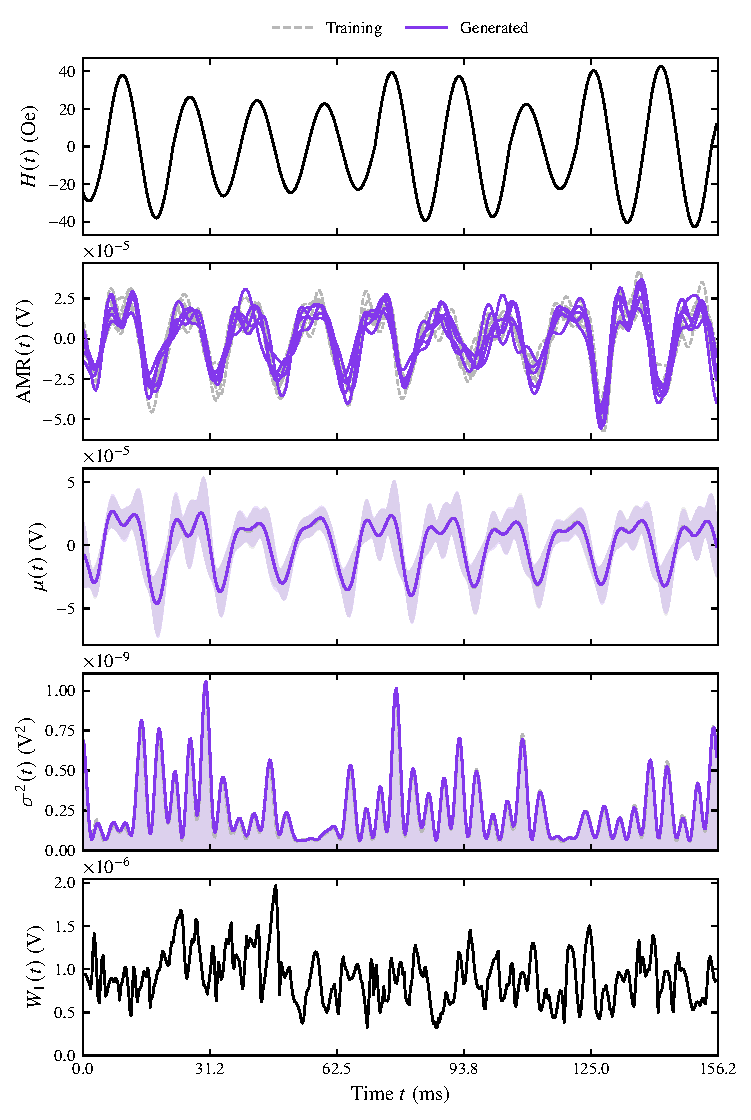
\includegraphics[width=0.9\linewidth]{amr.pdf}
\caption{}
\label{fig:amr}
\end{figure}

\subsection{Magnetoresistance with full-waveform conditioning}\label{ssec:amr}

The first dataset comprises magnetisation dynamics from an experimental spintronic device consisting of a lithographically patterned, interconnected array of permalloy
$\mathrm{Ni}_{80}\mathrm{Fe}_{20}$ nanoscale rings.  The array is driven by an in-plane rotating magnetic field with amplitude $H(t)$, and the resulting anisotropic magnetoresistance (AMR) is measured.\footnote{These dynamics provide the nonlinearity and fading memory required for reservoir computing~\cite{dawidek2021,vidamour2022,manneschi2025}.}  We refer the reader to Ref.~\cite{manneschi2025} for details of the device and measurement procedure.

Each AMR channel is modelled separately.  A training example is
\[
\left(\mathbf{q}^{(i)},\mathbf{h}^{(i)}\right),
\qquad
\mathbf{q}^{(i)},\mathbf{h}^{(i)}\in\mathbb{R}^{N_T},
\qquad
N_T=5000,
\]
where $\mathbf{q}^{(i)}$ is the measured AMR trajectory and $\mathbf{h}^{(i)}$ is the corresponding discretised field-amplitude waveform.  The raw measurements contain $100$ repetitions of each of $999$ field patterns.  After removing acquisition transients, each trajectory contains $5000$ samples, corresponding to $100$ cycles of $50$ samples at a sampling rate of $3200\,\mathrm{Hz}$.  The AMR is filtered using a fifth-order, zero-phase Butterworth band-pass filter from $40$ to $200\,\mathrm{Hz}$.  The field amplitude is represented as a stepwise conditioning signal, with one normalised value held constant over each $50$-sample cycle.  Ten repetitions per pattern are used, and the patterns are divided into training, validation, and test sets in an $80{:}10{:}10$ ratio. 

The conditional U-Net has hidden width $64$, kernel size $3$, and dilation factors $(1,2,4,8)$. The dilation schedule gives an effective receptive field of approximately $19$ field cycles, or $329\,\mathrm{ms}$, allowing the model to represent the long-range temporal correlations and coloured noise in the AMR signal. The trajectory length $N_T=5000$ is independent of the $1000$ algorithmic diffusion steps used during training.  The model is trained with noise-prediction mean-squared error and sampled using DDIM.

\subsection{Diffusion modelling of spectrograms: artificial spin ice}\label{ssec:asi}

The second dataset is obtained from an artificial-spin-ice (ASI) multilayer reservoir probed by ferromagnetic resonance (FMR) spectroscopy \cite{stenning2024neuromorphic}. The applied field, $H_{\mathrm{app}}(t)$, varies between approximately $180$ and $235\,\mathrm{mT}$, following either a Mackey--Glass or sinusoidal waveform. The measured response is $\mathrm{d}P/\mathrm{d}H$, recorded in arbitrary units across $N_F=201$ fixed frequency bins. Each trajectory is therefore a time--frequency matrix $\mathbf{Y}^{(i)}\in\mathbb{R}^{T\times201}$. The data were separated into experimental runs, divided into $T=50$-step windows with stride $10$, and split at the run level. This produced $359$ training and $84$ test windows for Mackey--Glass, and $448$ training and $104$ test windows for the sine wave. The field was globally $z$-scored, and each FMR channel was normalised using its training mean and standard deviation.

The data supplied to the diffusion model are multivariate one-dimensional time series. PCA was fitted to the training matrices after reshaping (from $[N_{\mathrm{train}},T,201]$ to $[N_{\mathrm{train}}T,201]$), so that each time slice was one observation and the frequency bins were the features. After mode-wise normalisation, the trajectories were rearranged to shape $K\times T$. We use $K=16$ modes, which explain $96.9\%$ of the Mackey--Glass variance.

The diffusion model receives these PCA modes and is conditioned on the input field. A one-dimensional residual U-Net convolves along the time axis; the 16 PCA modes are treated as jointly generated channels. The U-Net has three levels of dilation: $[1,2,4]$. The PCA is then inverted to reconstruct the full spectrogram.

This representation is suited to the available data. The Mackey--Glass training set contains only $359$ windows from $15$ experimental runs, and the stride-$10$ windows overlap. A two-dimensional image model would learn directly in the $50\times201=10{,}050$-value time--frequency space, with convolutions across both time and frequency. The PCA representation reduces the generated state to $16\times50=800$ values, which may capture the global correlations between the fixed frequency channels, and allows the U-Net to focus on temporal dynamics. It therefore provides a more data-efficient model for this small experimental dataset while retaining the full frequency response through inverse PCA. We observe that increasing the number of retained principal components beyond $K=64$ deteriorates training, for reasons we do not yet understand.
\section{Summary}
\label{sec:summary}

\texttt{diffusionsde} models a conditional distribution over discretised
stochastic trajectories. The package supports ancestral DDPM sampling and
reduced-step DDIM sampling. With $\eta=0$ and a fixed initial Gaussian tensor,
DDIM sampling is repeatable. The option \texttt{require\_grad=True} retains a
differentiable map from a conditioning parameter to a trajectory.

The call \texttt{DDPM()} constructs the model. The method \texttt{fit} learns a
conditional trajectory distribution, and \texttt{generate} samples an ensemble
for supplied conditions. The method includes data preparation, training, reverse
sampling, conversion to physical units, validation, and inverse estimation. The
Ornstein--Uhlenbeck case
provides analytic and finite-step references. The Duffing case tests nonlinear
transient dynamics with coloured forcing.

The method has clear limits. It requires sufficient trajectory coverage across the
conditioning domain; a low denoising loss alone does not establish physical
fidelity; and the current inverse solver matches pointwise moments rather than
temporal correlations. Validation must therefore include correlation and spectral
tests, and an inverse estimate must be interpreted together with conditioning
coverage and identifiability analysis.


\section*{Data availability}
Selected case studies (Ornstein--Uhlenbeck and Duffing) are reproduced end to end
by Jupyter notebooks distributed with the package. The experimental data are
available upon request. Code, notebooks, and configuration files are available at
\url{https://github.com/Neuromorphic-Spintronics/diffusion}.

\bibliographystyle{elsarticle-num}
\bibliography{refs}

\end{document}
